\chapter{Σχετική Βιβλιογραφία}
\label{ch:related_work}
Τα ερωτήματα εγγύτητας και η ανίχνευση σύγκρουσης διερευνώνται 
εκτενώς για δεκαετίες από ερευνητές στα γραφικά υπολογιστών, στη ρομποτική,
στις προσομοίωσες, την υπολογιστική γεωμετρία και τα κινούμενα σχέδια 
υπολογιστών. 
Εκτός από την ανίχνευση σύγκρουσης και τον υπολογισμό απόστασης, υπάρχει
σημαντική βιβλιογραφία σχετική με τις Ιεραρχίες Οριοθετικών Όγκων 
(\tl{BVH}) και τις διάφορες εφαρμογές τους. 
Σε αυτό το κεφάλαιο κάνουμε αναφορά σε άρθρα της βιβλιογραφίας 
που μελετούν το ίδιο ή παρόμοιο πρόβλημα με το δικό μας
και επισημαίνουμε τις τεχνικές που χρησιμοποιούνται 
και στη δική μας μεθοδολογία.

\section{Εύρεση Κοντινότερου Κόμβου από Σημείο}
\label{sec:nearest_node}
Αρχικά μελετάμε το παρακάτω πρόβλημα: \textit{"Δοθέντος ενός 
πλέγματος και ενός σημείου (\tl{query-point}), ζητείται να βρεθεί 
ο κοντινότερος προς το σημείο \textbf{κόμβος} του πλέγματος"}.
Το πρόβλημα αυτό ανάγεται στο κλασικό πρόβλημα εύρεσης των \textit{$k$ 
κοντινότερων γειτόνων} από ένα σύνολο σημείων (\tl{$k$NN}, όπου $k=1$). 

Για το πρόβλημα αυτό έχουν προταθεί διάφορες λύσεις. Για παράδειγμα 
η χρήση διαγραμμάτων \tl{Voronoi} στην περίπτωση δεδομένων 
με μικρό αριθμό διαστάσεων \cite{aurenhammer1991voronoi}.
Οι σημαντικότερες όμως συνεισφορές για το συγκεκριμένο πρόβλημα είναι 
αυτές του \cite{bentley1975multidimensional} με την εισαγωγή του 
\textit{\tl{kD-Tree}}, και του \cite{yianilos1993data} με την 
εισαγωγή του \textit{\tl{VP-Tree}} (βλ. για παράδειγμα το
\cite{simon1996fast} όπου γίνεται χρήση του \textit{\tl{kD-Tree}} για τον 
υπολογισμό του κοντινότερου κόμβου ενός τριγωνικού πλέγματος 
από σημείο).

Τα δύο παραπάνω δυαδικά δέντρα αναζήτησης απαιτούν $\bigO(n*logn)$
χρόνο προεπεξεργασίας των δεδομένων (για την κατασκευή τους
από το σύνολο των $n$ σημείων του τρισδιάστατου χώρου) και 
έπειτα $\bigO(logn)$ για την απάντηση ερωτημάτων κοντινότερου 
γείτονα, στη μέση περίπτωση. 
Στο ίδιο πλαίσιο εργασίας αναπτύσσεται ο πρώτος εκ των δύο αλγορίθμων που 
προτείνουμε, για το δικό μας πρόβλημα, όπου κατασκευάζουμε μια δομή 
δεδομένων και στη συνέχεια κάνουμε ερωτήματα κοντινότερου γείτονα 
για να υπολογίσουμε την απόσταση.

Πιο συγκεκριμένα, για την κατασκευή του \tl{\textit{kD-Tree}} το σύνολο 
των σημείων ενός κόμβου διχοτομείται σε δύο υποσύνολα που αποτελούν 
τα δύο παιδιά του κόμβου. Η διαδικασία αυτή επαναλαμβάνεται αναδρομικά:
\begin{itemize}
    \item Η διχοτόμηση γίνεται με βάση κάποιον άξονα ο οποίος εναλλάσσεται κυκλικά 
    (\tl{round-robin}) για τα διαδοχικά επίπεδα του δέντρου.
    Για παράδειγμα, στις τρεις διαστάσεις, ο διαχωρισμός γίνεται πρώτα με 
    βάση τον άξονα $x$, έπειτα με βάση τον άξονα $y$, έπειτα με τον $z$, 
    ξανά με βάση τον $x$ και ούτω καθεξής.
    \item Το κριτήριο για τον διαχωρισμό του συνόλου των σημείων $V$, ενός κόμβου, 
    σε δύο υποσύνολα $L$, $R$ είναι το εξής: Χωρίς βλάβη της γενικότητας 
    θεωρούμε πως ο άξονας διαχωρισμού είναι ο $x$. Αν $m$ είναι η διάμεσος 
    των $x$-συντεταγμένων των σημείων, τότε $L = \{p \in V \mid p_x \leq m \}$ 
    και $R = \{p \in V \mid p_x >= m \}$. 
    Τα σύνολα $L$, $R$ επιλέγονται ώστε να έχουν το ίδιο πλήθος στοιχείων 
    ή να διαφέρουν κατά ένα.
    Όμοια προκύπτει το κριτήριο και για τους άλλους άξονες.
    Η διάμεσος $m$ είναι πληροφορία που αποθηκεύεται για κάθε κόμβο του δέντρου
    και χρησιμοποιείται στα ερωτήματα εύρεσης του κοντινότερου γείτονα.
\end{itemize}

Έτσι προκύπτει ένα σχεδόν πλήρες, ισορροπημένο, δυαδικό δέντρο.
Οι ιδέες 1) της διχοτόμησης του συνόλου των δεδομένων με κυκλική εναλλαγή 
του άξονα διαχωρισμού και 2) η χρήση της διαμέσου των αντίστοιχων 
συντεταγμένων για τον διαχωρισμό  
χρησιμοποιούνται \textit{αυτούσιες} και στη δική μας μεθοδολογία 
για την κατασκευή μιας Ιεραρχίας Οριοθετικών Όγκων. 
Η διαφορά είναι πως χειριζόμαστε χωρικά δεδομένα, και όχι σημεία,
επομένως επιλέγεται ένα \textit{αντιπροσωπευτικό σημείο} για κάθε 
χωρικό αντικείμενο και εφαρμόζεται η ίδια μέθοδος κατασκευής της 
ιεραρχίας. 

\begin{wrapfigure}{l}{0.3\textwidth}
    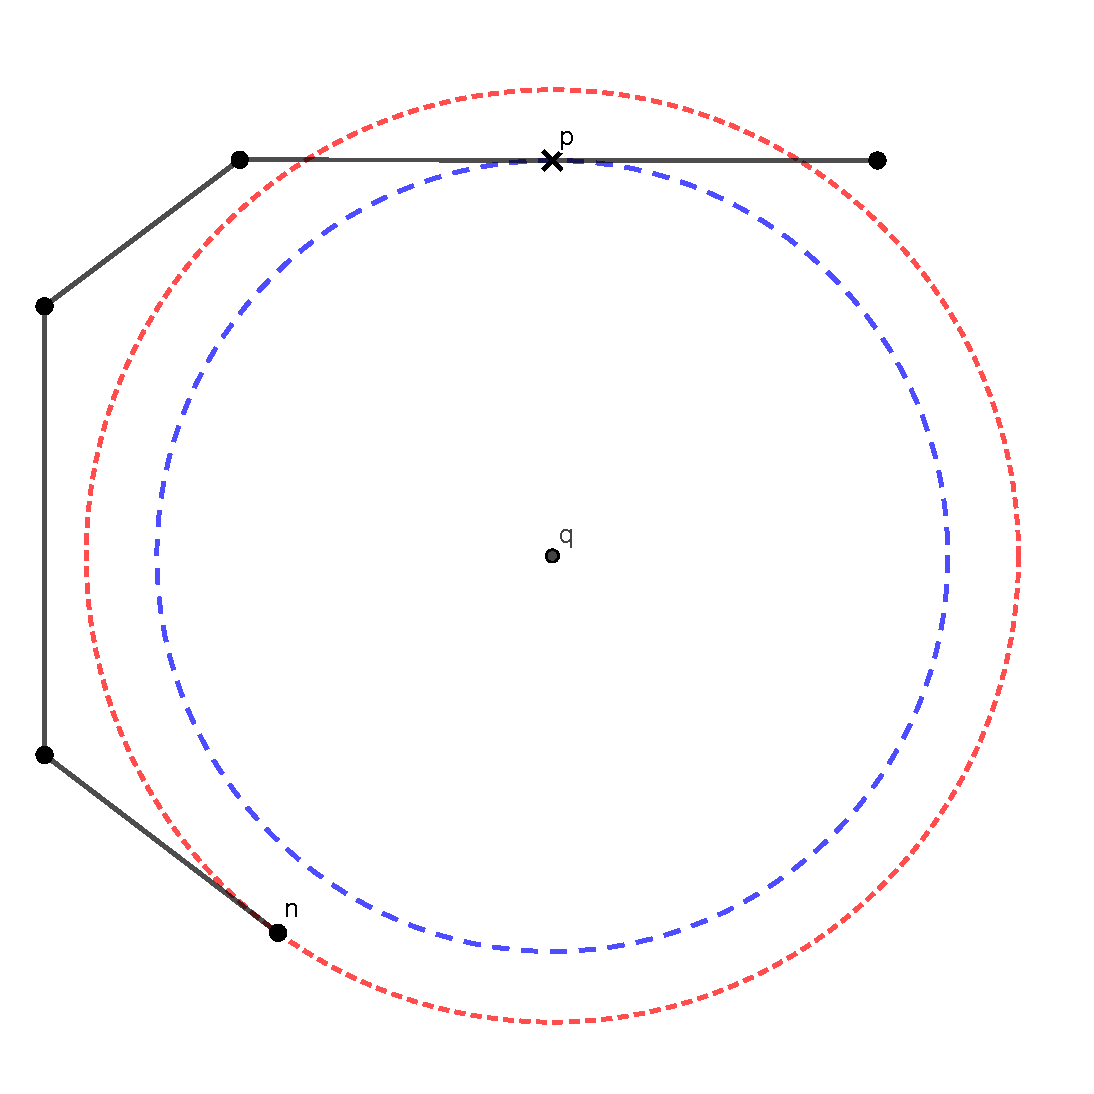
\includegraphics[width=0.29\textwidth]{nearest_node.pdf}
    \caption[Εύρεση Κοντινότερου Κόμβου από Σημείο]{
        Παράδειγμα όπου ο κοντινότερος \textit{κόμβος} $n$ ενός πλέγματος 
        διαφέρει από το κοντινότερο \textit{σημείο} $p$, δοθέντος 
        του \tl{query-point} $q$.}
    \label{fig:nearest_node}
\end{wrapfigure}

Για την κατασκευή του \tl{\textit{VP-Tree}}, ξανά, το σύνολο των σημείων 
ενός κόμβου διχοτομείται σε δύο υποσύνολα αναδρομικά:
\begin{itemize}
    \item Αρχικά, επιλέγεται ένα τυχαίο σημείο από το σύνολο $V$ των σημείων 
    του κόμβου. Το σημείο αυτό ονομάζεται \textit{\tl{vantage-point (vp)}} 
    και αποτελεί πληροφορία που αποθηκεύεται στον κόμβο.
    \item Έπειτα υπολογίζονται οι αποστάσεις όλων των υπολοίπων σημείων 
    προς το \tl{vp} και η διάμεσος $m$, που επίσης αποθηκεύεται στον κόμβο.
    \item Αν $m$ είναι η διάμεσος των αποστάσεων που υπολογίστηκαν 
    τότε το σύνολο του αριστερού παιδιού είναι το 
    $L = \{p \in V \mid distance(p,vp) \leq m \}$
    και του δεξιού παιδιού 
    $R = \{p \in V \mid distance(p,vp) \geq m \}$
\end{itemize} 

Ο τυπικός τρόπος για την απάντηση ερωτημάτων κοντινότερου κόμβου 
είναι, αρχικά, ο υπολογισμός μιας εκτίμησης αυτού διασχίζοντας το δέντρο 
από τη ρίζα έως κάποιο φύλλο. 
Το φύλλο αποτελεί την πρώτη εκτίμηση κοντινότερου κόμβου, ενώ η επιλογή του 
μονοπατιού από τη ρίζα μέχρι το φύλλο αποτελεί σχεδιαστική επιλογή και 
χρησιμοποιούνται ευρετικοί μέθοδοι (\tl{heuristics}).
Έπειτα μια σφαίρα εκτείνεται από το \tl{query-point} έως το φύλλο 
και, με τη βοήθεια του δέντρου, από τα υπόλοιπα σημεία ελέγχονται μόνο 
αυτά που βρίσκονται εντός της σφαίρας. 
Η ακτίνα της σφαίρας μικραίνει όσο ανακαλύπτονται όλο και κοντινότεροι 
κόμβοι.
Αυτή η διαδικασία λέγεται \textit{κλάδεμα (\tl{pruning})} του δέντρου,
και μειώνει τον χώρο αναζήτησης με το να απορρίπτει περιοχές που δεν 
μπορούν να περιέχουν τον κοντινότερο γείτονα. 
Με αυτόν τον τρόπο, ο αριθμός των αναμενόμενων συγκρίσεων 
είναι της τάξης $\bigO(logn)$ για τη μέση περίπτωση. 
Με ίδιο μοτίβο λογικής σχεδιάζεται και η διαδικασία αναζήτησης 
κοντινότερου γείτονα για χωρικά δεδομένα που προτείνουμε. 

Το παραπάνω πρόβλημα δεν πρέπει να συγχέεται με το πρόβλημα εύρεσης 
του κοντινότερου \textit{σημείου} ενός πολυγωνικού πλέγματος από 
κάποιο \tl{query-point}. Γενικά ο κοντινότερος \textit{κόμβος} και 
το κοντινότερο \textit{σημείο} ενός πλέγματος μπορούν να απέχουν 
πολύ μεταξύ τους όπως φαίνεται στο Σχήμα \ref{fig:nearest_node}:
Η πολυγωνική γραμμή αντιπροσωπεύει το σύνορο ενός υποθετικού πλέγματος 
στις δύο διαστάσεις και η ελάχιστη απόσταση του πλέγματος από το σημείο 
$q$ (ακτίνα του κόκκινου κύκλου) διαφέρει από την 
απόσταση του κοντινότερου κόμβου (ακτίνα του μπλε κύκλου).


% να πω για linear programming 
% These include Dobkin-
% Kirkpatrick hierarchies [DK82], linear programming [Sei90] and algorithms for intersecting
% convex p olytop es [Cha89 ] 
% και γενικά ό,τι αναφέρεται στο paper του GJK.

\section{Οργάνωση Χωρικών Δεδομένων σε Ιεραρχίες}
Η ιεραρχική οργάνωση των αντικειμένων του χώρου σε δενδρικές 
δομές δεδομένων αποτελεί κοινή μεθοδολογία για πολλά προβλήματα 
της Υπολογιστικής Γεωμετρίας. 
Τέτοιες δομές χρησιμοποιούνται σε διάφορες εφαρμογές για να 
επιταχύνουν τη διαδικασία επίλυσης του εκάστοτε προβλήματος, 
όπως ακριβώς συμβαίνει και στη μεθοδολογία που προτείνουμε. 
Για τον λόγο αυτό πολλές φορές αναφέρονται και ως \textit{δομές 
δεδομένων επιτάχυνσης (\tl{acceleration data structures})}.

Χαρακτηριστικά παραδείγματα αποτελούν:
\begin{itemize}
    \item Οι δομές \tl{\textit{VP-Tree}, \textit{kD-Tree}} που 
    περιγράφονται στο \ref{sec:nearest_node} και χρησιμοποιούνται 
    για το πρόβλημα εύρεσης των $k$ κοντινότερων γειτόνων (\tl{\textit{kNN}}). 

    \item Το \tl{\textit{R-Tree}} που περιγράφεται στο \cite{guttman1984r}, 
    και χρησιμοποιείται ως ευρετήριο σε βάσεις δεδομένων που αποθηκεύουν χωρικά 
    δεδομένα/αντικείμενα.
    Το \tl{R-Tree} χρησιμοποιεί \textit{ελάχιστα οριοθετικά παραλληλόγραμμα (\tl{MBR})}
    για την οργάνωση των χωρικών αντικειμένων, από τα φύλλα έως τη ρίζα και ανήκει 
    στην οικογένεια των Ιεραρχιών Οριοθετικών Όγκων (\tl{BVH}).
    Υποστηρίζει εισαγωγή, διαγραφή και ενημέρωση δεδομένων καθώς επίσης 
    και ερωτήματα εύρεσης των αντικειμένων που βρίσκονται εντός μιας δοθείσας περιοχής. 
    Γενικά, το \tl{R-Tree} δεν είναι δυαδικό δέντρο και ο τρόπος διάσχισης του 
    δεν είναι τετριμμένος.
    Στο \cite{roussopoulos1995nearest} περιγράφεται ένας αλγόριθμος 
    εύρεσης των $k$ κοντινότερων αντικειμένων από κάποιο σημείο $p$, για το \tl{R-Tree}.
    Στον αλγόριθμο αυτόν εισάγωνται οι μετρικές απόστασης \textit{\tl{MINDIST}}
    και \textit{\tl{MINMAXDIST}} βάση των οποίων ορίζεται η σειρά της αναζήτησης 
    με κάποια προτεραιότητα.
    Οι μετρικές αποτελούν το κάτω και άνω φράγμα, αντίστοιχα, της απόστασης του 
    αντικειμένου από το σημείο $p$.

    \item Το \tl{\textit{BSP-Tree}}, που περιγράφεται στο \cite{fuchs1980visible},
    χρησιμοποιείται για την απόδοση γραφικών καθώς μπορεί να δώσει χωρικές πληροφορίες 
    για τα αντικείμενα μιας σκηνής. 
    Συνήθως τα αντικείμενα είναι πολύγωνα στον τρισδιάστατο χώρο.
    Η δομή του επιτρέπει την εύκολη διάσχιση των αντικειμένων μιας σκηνής από πίσω προς 
    τα εμπρός για δοσμένη θέση θέασης.
    Συγκεκριμένα, η κατασκευή του γίνεται μια μόνο φορά για κάποια στατική σκηνή 
    και το ίδιο δέντρο μπορεί να χρησιμοποιηθεί για οποιαδήποτε γωνία θέασης.
    Για την κατασκευή του, ο χώρος διαχωρίζεται αναδρομικά 
    σε δύο ημι-χώρους (\tl{half-spaces}) με βάση κάποιο επίπεδο.
    Τα αντικείμενα (ολόκληρα ή κάποιο μέρος τους) τοποθετούνται στο αριστερό ή δεξί
    παιδί ανάλογα με τον ημι-χώρο στον οποίο ανήκουν.
    Παρόλο που αποθηκεύει χωρικά δεδομένα (και όχι σημεία), το \tl{BSP-Tree} 
    θεωρείται γενίκευση του \tl{kD-Tree} διότι τα επίπεδα που χωρίζουν 
    τον χώρο μπορεί να έχουν οποιονδήποτε προσανατολισμό σε αντίθεση 
    με τα ευθυγραμμισμένα με τους άξονες επίπεδα του \tl{kD-Tree}.

    \item Το \tl{\textit{Octree}}, που περιγράφεται στο \cite{meagher1982geometric}
    χρησιμοποιείται σε πολλές εφαρμογές για απόδοση γραφικών, ανίχνευση σύγκρουσης, 
    ανίχνευση ακτίνων, ως χωρικό ευρετήριο, ως γεννήτρια πλεγμάτων κ.α. 
    Ένας κόμβος του δέντρου μπορεί να έχει έως και οκτώ παιδιά που κάθε ένα
    αντιπροσωπεύει ένα ογδοημόριο του τρισδιάστατου χώρου που καταλαμβάνει ο 
    πατρικός κόμβος.
    Συνήθως για την κατασκευή του αρχικά ορίζεται το ελάχιστο μέγεθος που μπορεί να 
    έχει ένα ογδοημόριο και ο χώρος που καταλαμβάνει η ρίζα του δέντρου. 
    Έπειτα κάθε κόμβος του  δέντρου 
    διαιρείται σε ογδοημόρια μέχρι είτε να μην περιέχεται κανένα αντικείμενο 
    εντός του ογδοημορίου, είτε το ογδοημόριο να πάρει το ελάχιστο δυνατό μέγεθος.
    Οι κόμβοι του δέντρου που δεν περιέχουν τίποτα στο εσωτερικό τους μπορούν να αγνοηθούν.
    Έτσι, οποιοδήποτε τρισδιάστατο αντικείμενο μπορεί να αναπαρασταθεί με οσοδήποτε 
    μεγάλη ανάλυση (\tl{resolution}).
    Στην παραπάνω δημοσίευση περιγράφονται επίσης αλγόριθμοι για διάφορες πράξεις μεταξύ 
    αντικειμένων που αναπαρίστανται από \tl{Octrees}.
    Τέτοιες είναι οι πράξεις της ένωσης, τομής, διαφοράς, οι γεωμετρικές πράξεις 
    μεταφοράς, περιστροφής, κλιμάκωσης και η ανίχνευση σύγκρουσης και απόδοσης γραφικών 
    από οποιαδήποτε γωνία θέασης. 
\end{itemize}

Πολλές από τις τεχνικές που αναφέρονται παραπάνω ακολουθούνται και 
στη δική μας μεθοδολογία.
Παραδείγματα αποτελούν η χρήση οριοθετικών όγκων και η αναδρομική οργάνωση 
των αντικειμένων σε μια ιεραρχία, η μοντελοποίηση του προβλήματος 
ως πρόβλημα κοντινότερων γειτόνων για χωρικά δεδομένα και ο 
ορισμός της σειράς επίσκεψης των κόμβων της ιεραρχίας, κατά την αναζήτηση, με 
βάση μια μετρική απόστασης.

Τέλος, αξίζει να σημειωθεί ότι στη βιβλιογραφία γίνεται λόγος για την 
ποιότητα των Ιεραρχιών Οριοθετικών Όγκων. 
Ορίζονται μετρικές ποιότητας που χρησιμεύουν τόσο στην αξιολόγηση όσο 
και στην κατασκευή των ιεραρχικών δομών.
Επί του παρόντος, δεν υπάρχει πρακτικός τρόπος για τον προσδιορισμό 
του βέλτιστου διαχωρισμού των αντικειμένων ενός κόμβου σε δύο υποσύνολα.
Έτσι, δεν είναι γνωστό ποια αντικείμενα πρέπει να ομαδοποιηθούν μαζί
με άλλα για να επιτευχθεί η καλύτερη δυνατή επίδοση των αλγορίθμων.
Η πιο διαδεδομένη μετρική κόστους είναι η 
\textit{\tl{SAH (Surface Area Heuristic)}} 
\cite{goldsmith1987automatic} \cite{macdonald1990heuristics}
η οποία, περιληπτικά, "επιβραβεύει" μικρούς χωρικά κόμβους με πολλά 
αντικείμενα και "τιμωρεί" μεγάλους κόμβους με λίγα τρίγωνα. 
Επίσης, στο \cite{aila2013quality} εισάγωνται οι μετρικές 
\tl{\textit{EPO (End-point Overlap)}} και 
\tl{\textit{LCV (Leaf Count Variability)}} ως συμπληρωματικές 
της \tl{SAH} για να εξηγήσουν την παρατηρούμενη επίδοση 
των δέντρων σε περιπτώσεις όπου η \tl{SAH} αδυνατεί να 
δικαιολογήσει την επίδοση κάποιων δέντρων συγκριτικά 
με άλλα.

% Απόσταση Σημείου από Πολυγωνικό Πλέγμα
% Απόσταση Δύο Πολυγωνικών Πλεγμάτων
% Απόσταση Αντικειμένων που Περιγράφονται από \tl{NURBS}
